%=========================================================
% 32bit ISA Specifications
%=========================================================
\section{32bit ISA Specifications}

\begin{table}[H]
    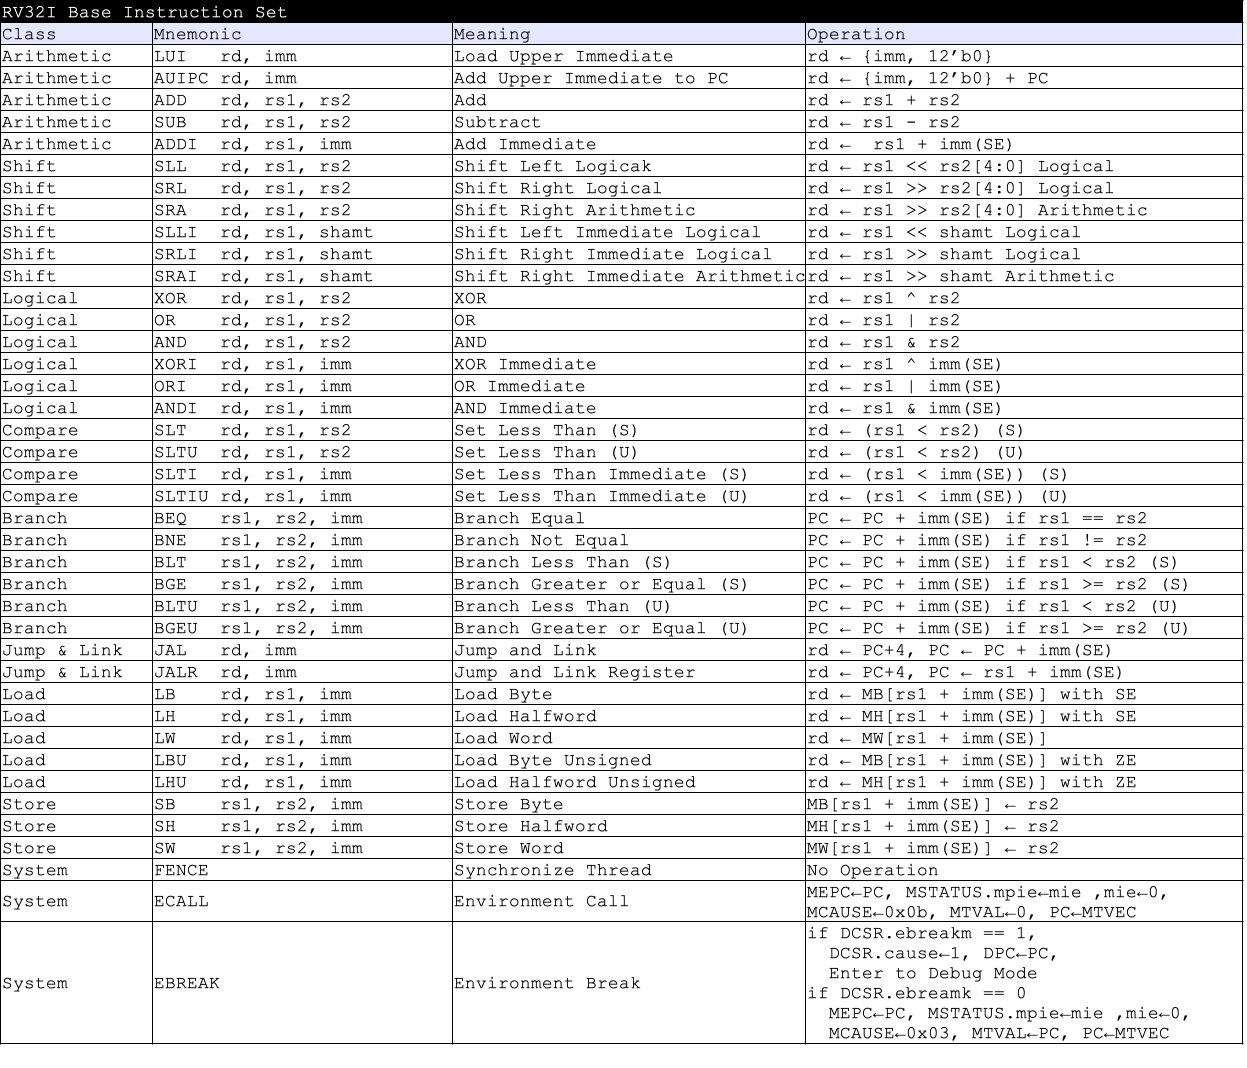
\includegraphics[width=1.00\columnwidth]{./Table/ISASpec_RV32I.png}
    \caption{RV32I Base Instruction Set Specification}
    \label{tb:ISASpec_RV32I}
\end{table}

\begin{table}[H]
    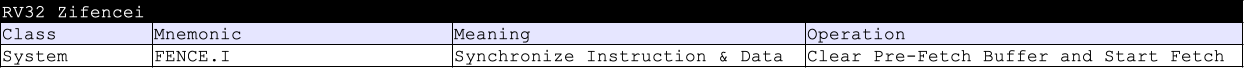
\includegraphics[width=1.00\columnwidth]{./Table/ISASpec_RV32Zifencei.png}
    \caption{RV32 Zifencei Specification}
    \label{tb:ISASpec_RV32Zifencei}
\end{table}

\begin{table}[H]
    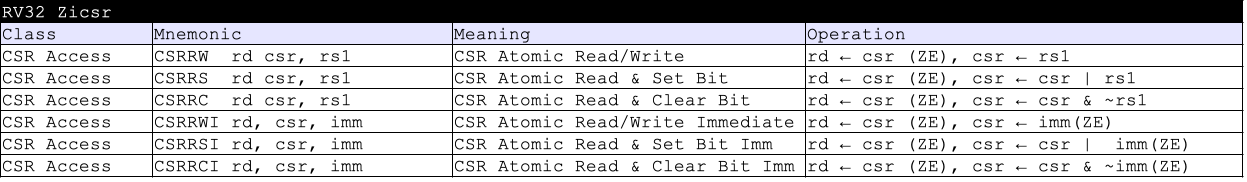
\includegraphics[width=1.00\columnwidth]{./Table/ISASpec_RV32Zicsr.png}
    \caption{RV32 Zicsr Specification}
    \label{tb:ISASpec_RV32Zicsr}
\end{table}

\begin{table}[H]
    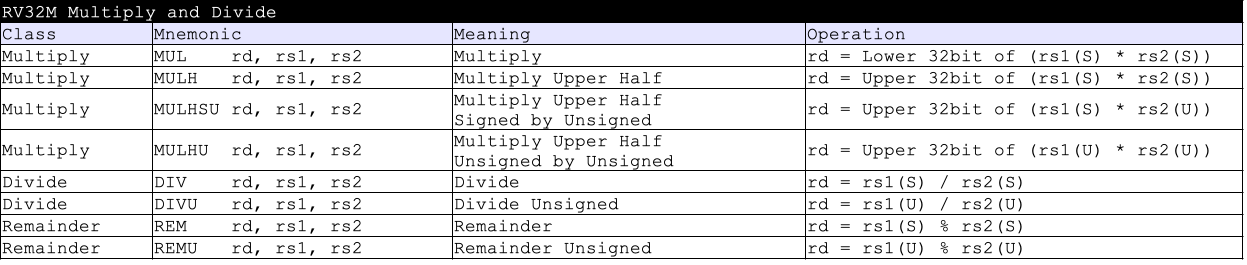
\includegraphics[width=1.00\columnwidth]{./Table/ISASpec_RV32M.png}
    \caption{RV32M Multiply and Divide Specification}
    \label{tb:ISASpec_RV32M}
\end{table}

\begin{table}[H]
    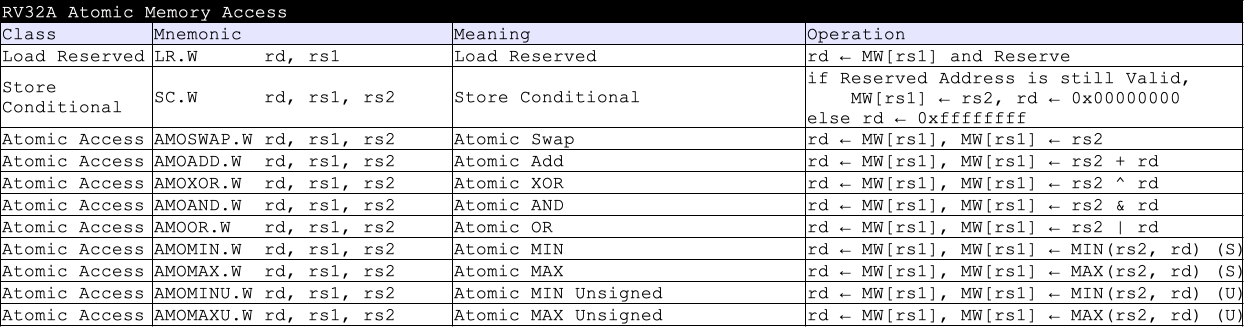
\includegraphics[width=1.00\columnwidth]{./Table/ISASpec_RV32A.png}
    \caption{RV32A Atomic Memory Access Specification}
    \label{tb:ISASpec_RV32A}
\end{table}

\begin{table}[H]
    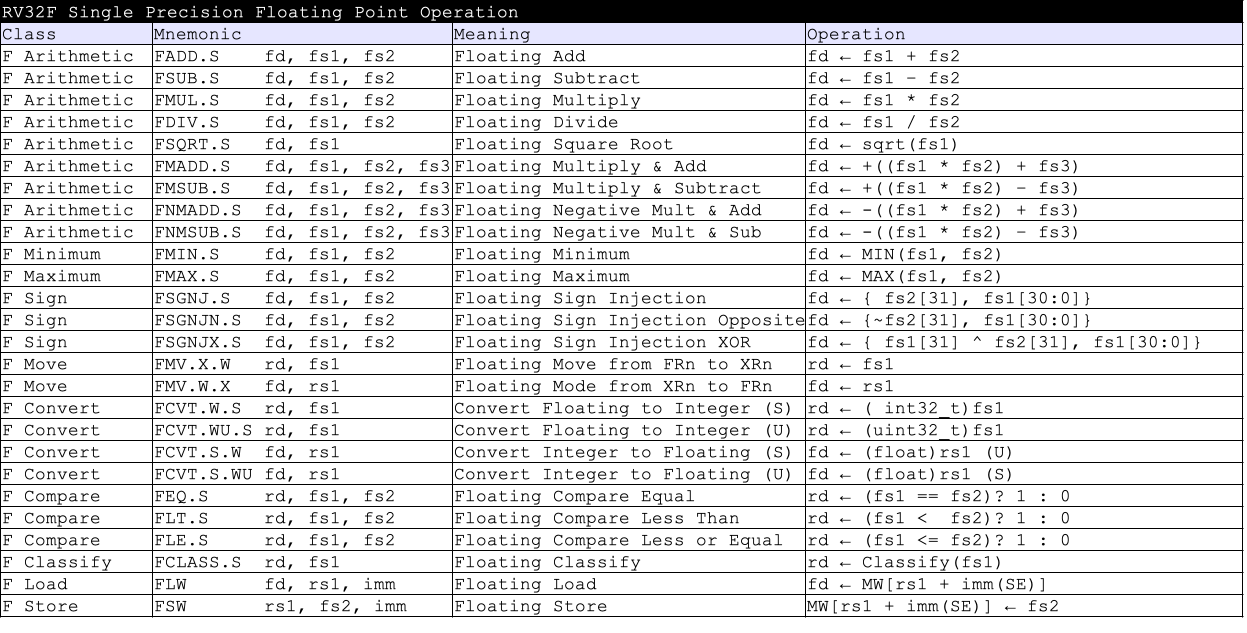
\includegraphics[width=1.00\columnwidth]{./Table/ISASpec_RV32F.png}
    \caption{RV32F Single Precision Floating Point Operation Specification}
    \label{tb:ISASpec_RV32F}
\end{table}

\begin{table}[H]
    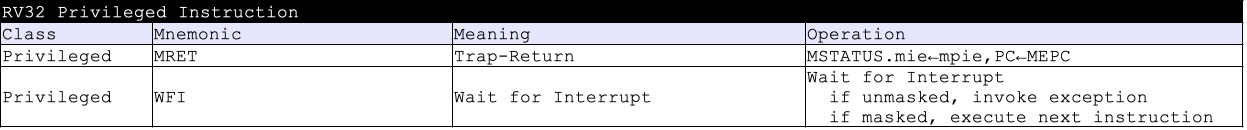
\includegraphics[width=1.00\columnwidth]{./Table/ISASpec_RV32Priviledged.png}
    \caption{RV32 Privileged Instruction Specification}
    \label{tb:ISASpec_RV32Priviledged}
\end{table}

The WFI (Wait for Interrupt) Instruction waits for interrupt requests. If the received interrupt is enabled, an exception corresponding to the interrupt starts. If the received interrupt is not enabled (masked by mie = 0), the CPU resumes and starts from the next instruction after WFI.





